% section Evaluation
\label{sec:eval}


We now present the experimental evaluation of our caching-based keep-alive and provisioning techniques by using function workload traces and serverless benchmarks.
Our goal is to investigate the effectiveness of the these techniques under different workload and system conditions. 


\begin{figure*}
  \centering
    \vspace*{\myfigspace}
\subfloat[ Representative functions.     \label{fig:rep-trace-exec}]
{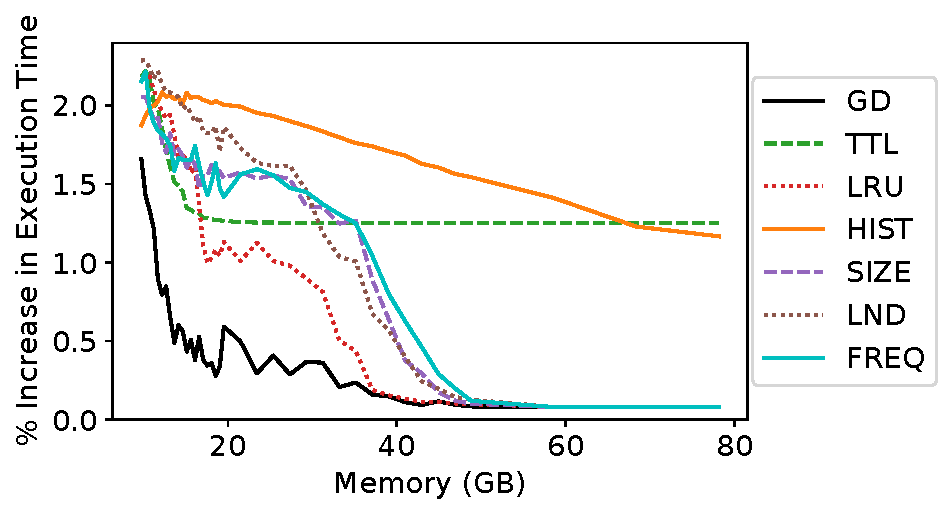
\includegraphics[width=0.37\textwidth]{../graphs/rep-funcs-392/exec_inc_mem-392-legend.pdf}}
  \hfill 
    \subfloat[Rare functions.     \label{fig:rare-trace-exec}]
{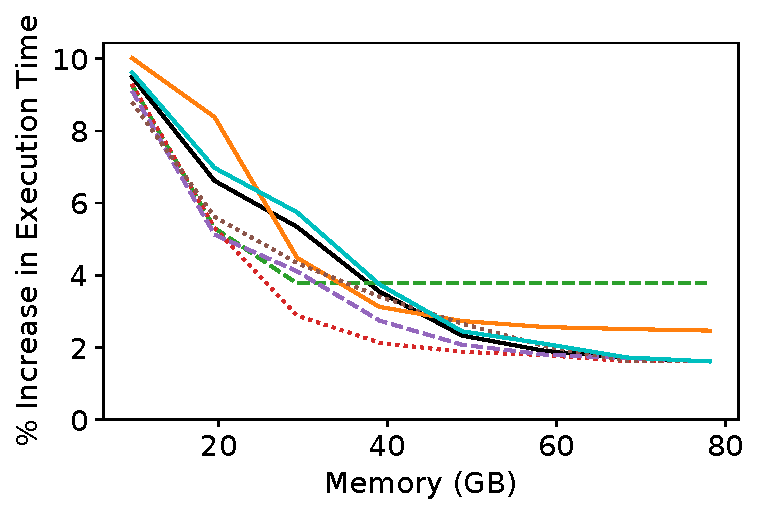
\includegraphics[width=0.3\textwidth]{../graphs/rare-funcs-1000/exec_inc_mem-1000.pdf}}
\hfill 
  \subfloat[Random sampling.      \label{fig:random-trace-exec}] {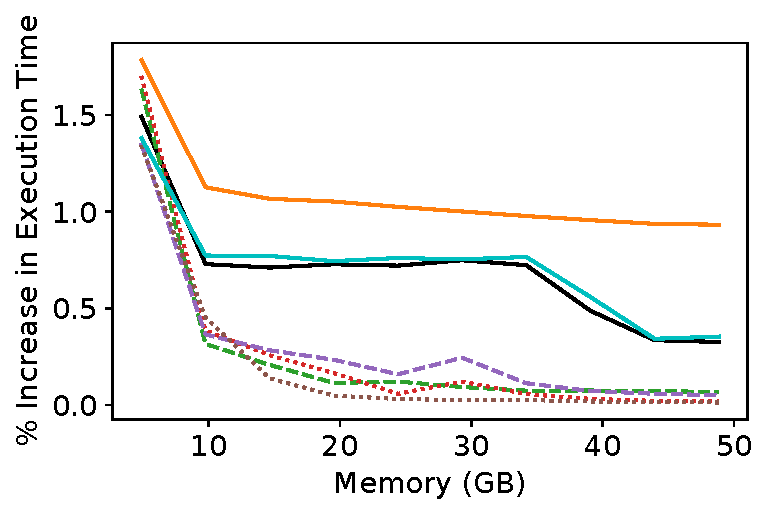
\includegraphics[width=0.3\textwidth]{../graphs/random-funcs-200/exec_inc_mem-200.pdf}}
  \vspace*{\myfigspace}
\caption{Increase in execution time due to cold starts for different workloads derived from the Azure function trace.}
\label{fig:exec-overheads-all}
  \vspace*{\myfigspace}
\end{figure*}


\begin{figure*}[t]
  \centering
%  \vspace*{\myfigspace}
%  \begin{minipage}[c]{0.7\linewidth}
  \subfloat[Representative functions.\label{fig:rep-trace-cold}] {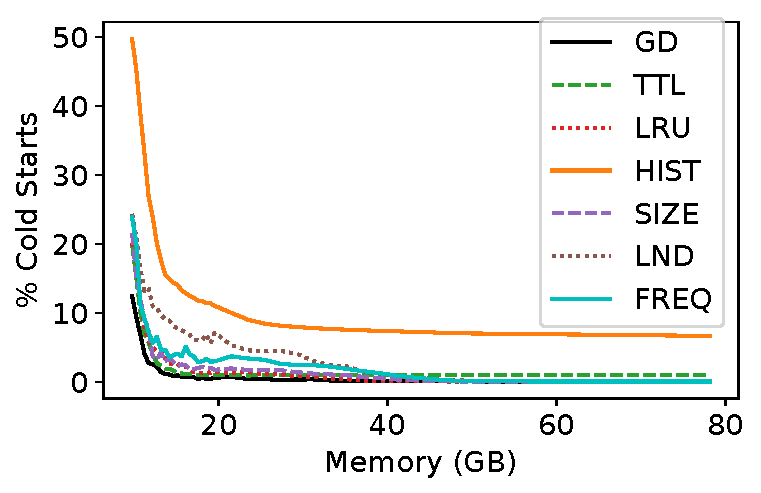
\includegraphics[width=0.33\textwidth]{../graphs/rep-funcs-392/cold_drop_mem-392-legend.pdf}}
  \hfill
    \subfloat[Rare functions. \label{fig:rare-trace-cold}] {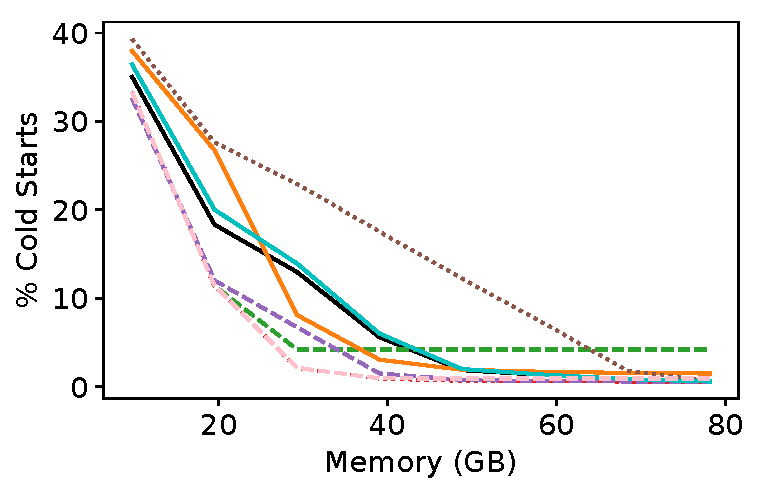
\includegraphics[width=0.33\textwidth]{../graphs/rare-funcs-1000/cold_drop_mem-1000.pdf}}
  \hfill
  \subfloat[Random sampling. \label{fig:random-trace-cold}]
  {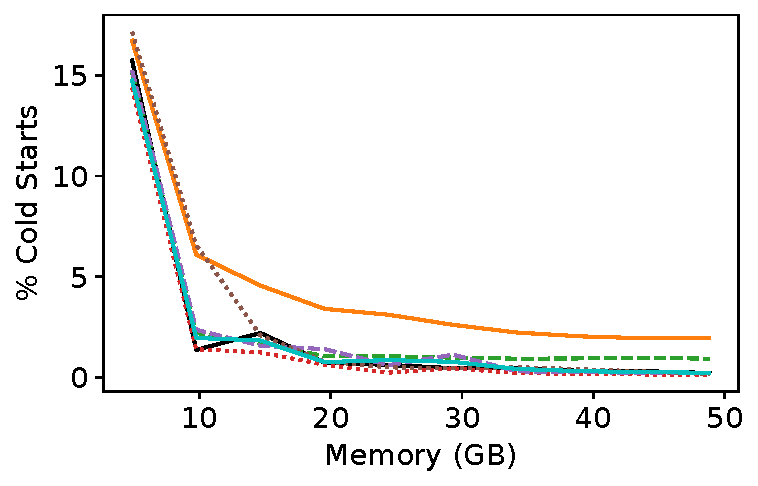
\includegraphics[width=0.33\textwidth]{../graphs/random-funcs-200/cold_drop_mem-200.pdf}}
    \vspace*{\myfigspace}
    \caption[cold starts]{Fraction of cold starts is lower with caching-based keep-alive. } % for different samples of the Azure function trace.}
      \vspace*{\myfigspace}
      \label{fig:cold starts-all}
%    \end{minipage}
%    \hfill
%    \begin{minipage}[c]{0.29\linewidth}
 %      \begin{figure}
 %     \end{figure}
%    \end{minipage}
\end{figure*}


%%%%%%%%%%%%%%%%%%%%%%%%%%%%%%%%%%%%%%%%%%%%%%%%%%%%%%%%%%%%
\noindent \textbf{Setup, Workloads, and Metrics.}
%
For evaluating different keep-alive performance with different workload types, we use different trace samples from the Azure Function trace~\cite{shahrad_serverless_2020}, which contains execution times, memory sizes, and invocation-timestamps for more than 50,000 unique functions. 
Since our goal is to examine performance at a \emph{server} level, we use smaller samples of this trace for realistic server sizes, and replay them in our discrete-event keep-alive simulator. 
This also allows us to examine the behavior with different \emph{types} of workloads, which is important because our keep-alive policies are designed to be general and workload-agnostic.
We use the following three trace samples (more details in the Table~\ref{tab:trace-deets}): \\
\noindent \textbf{RARE:} A random sample of 1000 of the rarest, most infrequently invoked functions. These functions will usually result in cold starts under a classic 10 minute TTL.  \\
% mention 75% percentile detail?
\noindent \textbf{REPRESENTATIVE:} A sample of 400 functions, sampled from each quartile of the dataset based on frequency---yielding a more representative sample with higher function diversity. \\
\noindent \textbf{RANDOM:} A random sample of 200 functions.

The FaasCache system is evaluated in Section~\ref{subsec:ow-eval}.
Functions from the FunctionBench~\cite{kim_functionbench_2019} suite are used for generating a realistic workload. 
A single server with 250 GB RAM and 48-core Intel Xeon Platinum 2.10 GHz CPUs is used for running all functions. The server is running modified OpenWhisk (i.e., FaasCache), and Ubuntu 16.04.5. 

\begin{table}
  \caption{Size and inter-arrival time (IAT) details for the Azure Function workloads used in our evaluation.}
  \begin{tabular}{lrrr}
    \hline 
    Trace & Num Invocations & Reqs per sec & Avg. IAT \\
    \hline
    Representative & 1,348,162 & 190 /s & 5.4 ms \\
    Rare & 202,121 & 30 /s & 36 ms \\
    Random & 4,291,250 & 600 /s & 1.8 ms \\
    \hline
  \end{tabular}
  \label{tab:trace-deets}
\end{table}



\paragraph{Adapting the Azure Functions Trace.}
The format of the original Azure Function trace~\cite{shahrad_serverless_2020} requires some additional pre-processing and extrapolation for generating a workload.  
The full dataset consists of 14 days of function invocations, and billions of individual invocations. We use the first day's data, and do not consider functions that are never reused (i.e., with less than two invocations). 

The original trace provides memory consumption at the \textit{application} level---with the application made up of multiple functions.
Therefore, we evenly split the memory allocation between all functions in an application.
The dataset provides invocations in minute-wide buckets.
When injecting/replaying the workload, if there is only one invocation in a minute-bucket, it is injected at the beginning of the minute. 
For multiple invocations, they are equally spaced throughout the minute. 

%
The cold start overhead of each function is estimated as {\texttt maximum - average} runtime, and the execution times provided in the dataset are used for this computation. 
The dataset does not account for certain important sources of cold start overheads such as execution environment creation (e.g., Docker).
This unfortunately underestimates the cold start overheads.
However, because it applies uniformly to all functions, it preserves the relative performance of the different keep-alive policies, and does not affect the cache hit ratios. 
%

%These cold start overheads are generally constant, 

%This may not capture all the sources of cold start overhead such as the execution environment creation (e.g., Docker) and 

We are interested in two metrics: the cold start ratio; and the average increase in the execution time due to cold starts.
The increase in execution time is computed by averaging across all function invocations. 

%The latter captures the heterogeneity in function initialization overheads and invocation frequencies. 
%For estimating the time each function spends in explicit initialization, using the workload trace we subtract each functions' average runtime from its maximum runtime. 
%The dataset timings do not include provider overhead, so this initialization time is entirely due to application code.

%%
%Provider cold start overheads can be up to several seconds long, and take up the plurality of a function's execution time.
%Because the dataset does not include provider overhead, it is impossible to assign a realistic number to this cost.
%With these large penalties are not in our simulations, we therefore assume it as 0, but in reality the overhead is roughly constant.
%This causes the global increase in execution time to be smaller than it would be otherwise.
%Including a non-zero cold start cost would apply uniformly across all functions, and thus not change eviction priorities relative to one another.
%The cache hit ratio in Figure~\ref{fig:cold starts-all} would remain unchanged, and the Y-axis (the global increase in execution time) of Figure~\ref{fig:exec-overheads-all} would be scaled up relative to the chosen cold start overhead.
%%

% Using variable, real-world, times would require knowing or randomly assigning the runtime of functions, and would still require stochasticity as provider latency is not constant. 

% Not explaining this in the paper was our biggest “oops”: and there’s a few sources of confusion.
% Here is what we assumed: the dataset doesnt include container startup time, but the included function execution time captures both the function-initialization time (importing packages etc.), and the actual execution.
% So the assumption is that the Max execution time was due to this initialization overhead (which we include in the cold start overhead in our paper).
% The “time functions take to execute after they are ready to run” added to our confusion: we assumed this meant that it is the time when the control is transferred to the FaaS runtime inside the container: which would still incorporate all actual function initialization overheads.
% A contributing factor to making this assumptions was that most OpenWhisk applications do not have a strict explicit initialization, so it is in general not possible to know when a function is truly ready to execute non-idempotent code. 

% And so we end up with pretty small startup overheads, which can be seen from our Figure 5.
% Including container startup time and other overheads would make little difference to relative performance, since the extra overhead would apply to all functions.
% For instance, adding a constant startup penalty for all functions doesnt change their eviction priorities.
% The cache hit ratio (our Figure~\ref{fig:cold starts-all}) would remain unchanged, and the Y-axis of Figure~\ref{fig:exec-overheads-all} would be scaled up depending on the chosen cold start overheads. 

\begin{comment}
Our simulator evaluation uses real-world FaaS usage data from the recently released Azure Function trace~\cite{shahrad_serverless_2020}. 
The entire trace consists of tens of thousands of functions with billions of invocations, making it intractable to simulate the entire dataset.
Trace sampling methodology is important to capture the characteristics of the overall trace, and the scenarios where FaasCache is most effective.
Over half of all functions have an interval arrival time (IAT) over 30 minutes, where IAT is defined as execution time + idle time, guaranteeing them to always have cold starts when using a simple TTL eviction policy.
A tiny 1\% of functions account for nearly 90\% of all invocations, with an IAT of under a minute. 
% Therefore, smaller samples 
Given these extreme disparities, smaller samples must match behaviors of the larger dataset to show their effectiveness.
The full Azure trace can be suitably handled by a cluster of servers, in which case the system behavior is influenced by load-balancing and sharding policies, which our work is orthogonal to.
%Explain the rationale here. 
We generate three day-long traces using the Azure Functions dataset to showcase the effectiveness of FaasCache.
\prat{Insert reuse distance vs. time heatmaps for all these traces in the appendix along with table describing: number of fns, total invocations, avg. inter arrival time, etc.}
\end{comment}

%%%%%%%%%%%%%%%%%%%%%%%%%%%%%%%%%%%%%%%%%%%%%%%%%%%%%%%%%%%%
\subsection{Trace-Driven Keep-Alive Evaluation}
\vspace*{\subsecspace}
In this subsection, we use the Azure function traces to evalaute different keep-alive policies in our discrete-event simulator. 
% Primary Comparison? Competitors? 
We compare all caching-based variants against the default keep-alive policy in OpenWhisk (10 minute TTL).
% rev 1
When the server is full, this TTL policy evicts containers in an LRU order.
We also evaluate different Greedy-Dual variants: GD is our GDSF policy described in Section~\ref{subsec:gdsf}.
The others are the caching-based variants described in Section~\ref{subsec:variants}: LND is Landlord, and FREQ is LFU. 


%rev 1 
We also compare against the histogram based keep-alive policy in~\cite{shahrad_serverless_2020}, which is the state of the art technique.
% Section 4.2 of serverless paper 
We have reproduced this policy (HIST) from the details in the paper, and have implemented it in a ``best-effort'' manner without any knowledge of the optimizations in the actual implementation.
This is effectively a ``TTL+Prefetching'' policy: it uses a histogram of \emph{inter-arrival times} to predict future function invocations and eagerly evict warm functions.
It uses timeseries-forecasting to capture temporal locality, but does not consider the other function characteristics such as function size and initialization cost. 
The IAT, computed by taking a function's execution time plus the subsequent idle time, between each actual invocation is recorded in minute granularity buckets, tracking up to four hours between executions.
The policy uses ARIMA modeling for those invocations that fall outside this four hour window, we chose not to implement this specific feature due to its complexity, and the fact that it accounted for a minor fraction (\textasciitilde 0.56\%) of all invocations.
From these buckets, a function's coefficient of variation (CoV) is calculated using Welford's online algorithm~\cite{welford}. 
When the function's IAT is predictable (CoV $\leq 2$), the function's historical/customized preload and TTL time are used. Otherwise the function has a generic TTL of two hours. 
When an invocation is anticipated, it is brought into memory and kept there until its TTL expires.
A function is evicted when the policy predicts it will not have an invocation in the near future. 
%We chose not to implement the ARIMA modeling for IAT's exceeding four hours for simplicity and the fact it is only applicable to a tiny number of functions.
% \textbf{More details. Histogram size? When created? Online? }


%
The increase in execution time for different traces and for different cache sizes is shown in Figure~\ref{fig:exec-overheads-all}.
% How is this measured?
The increase in execution time is the cold start overheads averaged across all invocations of every function, and captures the user-visible response-time. 
%

For the representative trace (Figure~\ref{fig:rep-trace-exec}), Greedy-Dual reduces the cold start overhead by more than $3\times$ compared to TTL for a wide range of cache sizes (15--80 GB). 
Interestingly, it is able to achieve a low overhead of only 0.5\% at a much smaller cache size of 15GB, compared to other variants, which need 50 GB to achieve similar results---a reduction of cache size by more than $3\times$. 
%
For rare functions (Figure~\ref{fig:rare-trace-exec}), caching-based approaches such as LRU  reduce the cold start overhead by $2\times$ compared to TTL for cache sizes of 40--50 GB. 
This shows that for rare functions, recency is a more pertinent characteristic, and the complex four-way tradeoff used in Greedy-Dual is not necessarily ideal in all workload scenarios. 
For this workload, the HIST policy outperforms TTL, as reported in~\cite{shahrad_serverless_2020}. 
However, it results in 50\% higher cold start overhead compared to caching-based approaches.
Furthermore, because HIST uses only inter-arrival times, it is unable to perform well with heterogeneous representative workloads  (Figure~\ref{fig:rep-trace-exec}). 


Finally, the randomly sampled trace has a large number of infrequent functions because of the low probability of selecting the heavy-hitting functions.
In Figure~\ref{fig:random-trace-exec}, the recency component again dominates, and we see LRU outperforming other variants. 
The equivalence of LRU and TTL-based caching for rare objects has been noted~\cite{basu2017adaptive,jiang2018convergence}, which explains their similar behavior seen in Figure~\ref{fig:random-trace-exec}. 
%closeness of TTL and LRU performance for rare functions in our result. 


\noindent \emph{\textbf{Result:} For representative, diverse workloads, our GD policy can improve the performance and shrink cache sizes by up to $3\times$. For more homogeneous workloads, LRU can outperform current TTL-based approaches by $2\times$.}

%%%
% rev 1 
We can observe from Figure~\ref{fig:exec-overheads-all} that the increase in execution time is generally small ($<10\%$).
This is because of two main factors: the evaluation metric chosen, and the properties of the workload trace. 
The execution time is averaged across \emph{all} function invocations.
However, serverless workloads consists of a large number of very frequently invoked functions. 
The performance of these functions is generally not affected by keep-alive policies, since any policy is going to keep them in the cache because of their high frequency. 
Thus, the difference between non work-conserving policies such as TTL and Greedy-Dual is masked because of the frequent and popular functions. 
For instance, the average inter-arrival time for all three workloads is less than 36ms, or about 27 function invocations per second. 
Thus the server is overloaded, and TTL does well even though it is not work-conserving. 
As the IAT grows, the effectiveness of work-conserving caching-based approaches increases compared to TTL, as we shall see in the next subsection. 

%%%%
%While Figure~\ref{fig:exec-overheads-all} focuses on the average increase in execution latency, keep-alive can also reduce the tail latency of functions. Cold start 

%%%%

We see a similar relation and behavior in the miss-ratio curves shown in Figure~\ref{fig:cold starts-all}. 
Due to function heterogeneity, the cold start overheads are not strictly correlated with cache miss ratios, and thus the differences between policies is different compared to the previously described actual cold start overheads. 
% \prat{Write after colors are fixed.}
Classic miss-ratio curves do not consider the miss \emph{cost} (i.e., initialization cost), which is an important metric that is optimized by the Greedy-Dual approach.
Thus in general, even in object caching contexts, miss-ratio curves deviate from the actual performance---a behavior that we also observe. 

%%%%%%%%%%%%%%%%%%%%%%%%%%%%%%%%%%%%%%%%%%%%%%%%%%%%%%%%%%%%
\subsection{OpenWhisk Evaluation}
\label{subsec:ow-eval}
\vspace*{\subsecspace}


\begin{figure}
  \centering
  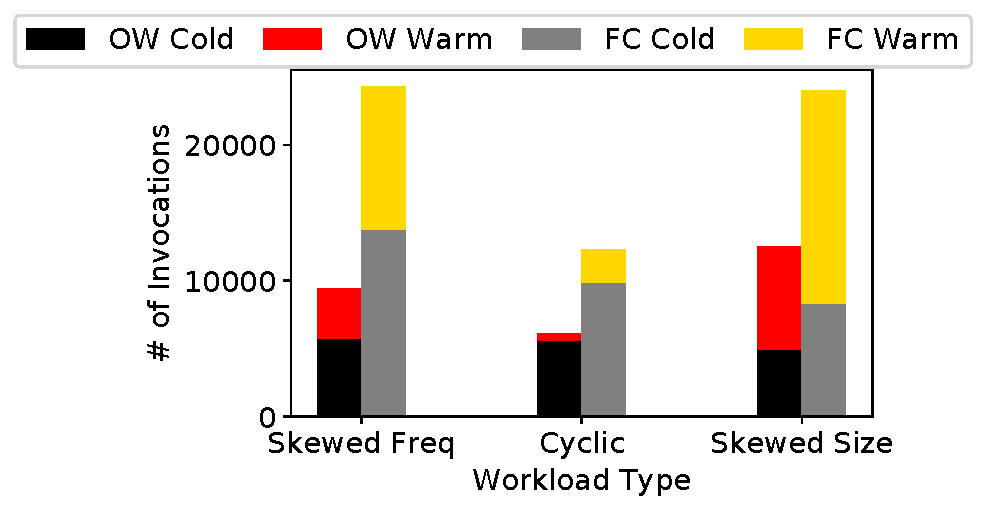
\includegraphics[width=0.47\textwidth]{../graphs/litmus_tests/litmus_2_stacked.pdf}
  \caption{FaasCache runs 50 to 100\% more cold and warm functions, for skewed workload traces.}
  \label{fig:litmus_2}  
\end{figure}


In this subsection, we evaluate the performance of the FaasCache system on real functions. 
We focus on the performance of FaasCache's Greedy-Dual keep-alive implementation, and compare it to the vanilla OpenWhisk system which uses a 10 minute TTL.


% rev1 1
In contrast to the previous subsection in which we showed the average performance for different cache sizes, we will now also focus on the inverse problem: for a fixed server size, how much more load can be handled with FaasCache? 
By leveraging Greedy-Dual caching, FaasCache is able to reduce cold starts. 
This also reduces the number of \emph{dropped} requests. %

OpenWhisk buffers and eventually drops requests if it cannot fulfill them.
Because FaasCache more effectively selects evictions, its higher hit rate results in functions finishing faster, allowing more functions to be executed in the same time frame.  
%
To examine the effect of Greedy-Dual keep-alive on cold start and dropped requests, we use a workload trace comprising of four different functions: Disk-bench, ML inference, Web-serving, and Floating-point from Table~\ref{tab:workloads}.

In Figure~\ref{fig:litmus_2}, we use different kinds of \emph{skewed} workloads: with a single function having a different frequency, a cyclic access pattern, and a skewed workload with 2 sizes. 
We see that FaasCache's keep-alive can increase the number of warm invocations by between 50 to 100\% compared to OpenWhisk's TTL.
The difference in the total number of requests served (warm+cold) is because OpenWhisk drops a significant number of requests due to its high cold start overhead and resultant system load. 
%
Thus with FaasCache, the total number of requests that are served also increases by $2\times$. 

%rev 1 above 
%Interestingly, OpenWhisk drops a significant number of requests, which is the cause of the different total served requests. 
%

% The impact on the different function performances can be seen in Figure~\ref{fig:faasbench}.
% For this figure, to generate the workload, the first three functions have an inter-arrival time of 1500 ms, and the fourth (floating-point) has a lower IAT of 400 ms. 

%a disk-based one, web-page serving, floating-point trigonomotry operations in numpy, and a convolutional neural network inference (TensorFlow with which model?). % A detailed description of these workloads is required.

% Explain what is the iat distribution and (other details? ).


% 32 GB wted_increase vanilla 11.964% cache 11.528%
% 48 GB wted_increase vanilla 6.184% cache 0.624%


\begin{figure}[t]
  \centering
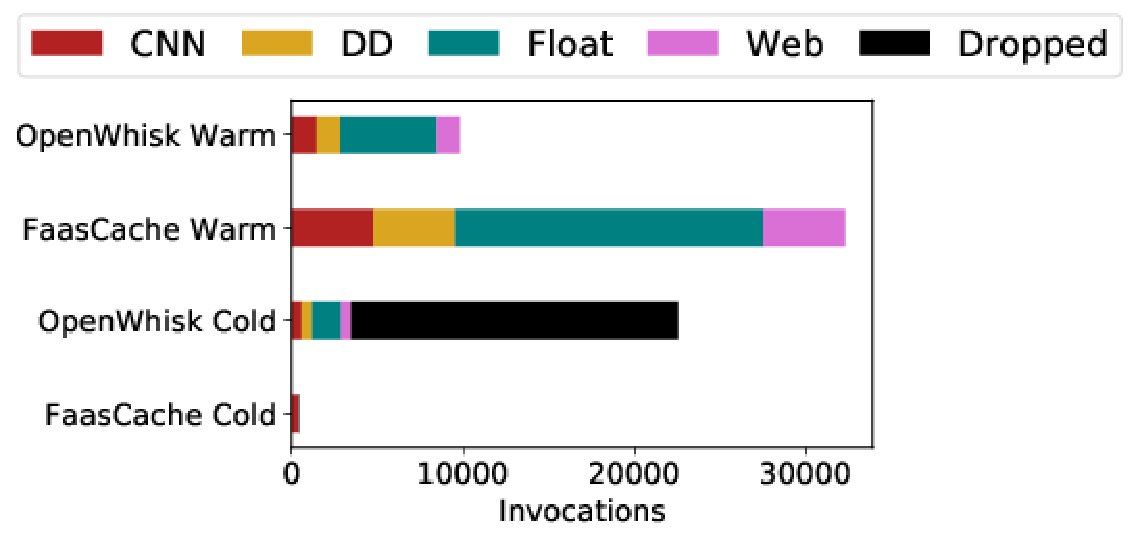
\includegraphics[width=0.47\textwidth]{../graphs/litmus_tests/faasbench_48_cold_hot-legend.pdf}
\caption{FaasCache increases warm-starts by more than $2\times$, which also reduces system load and dropped functions.}
\label{fig:faasbench}
\end{figure}


\begin{comment}
\begin{figure}[t]
  \centering
\subfloat[48 GB   \label{fig:faasbench-stacked-48}]
{ 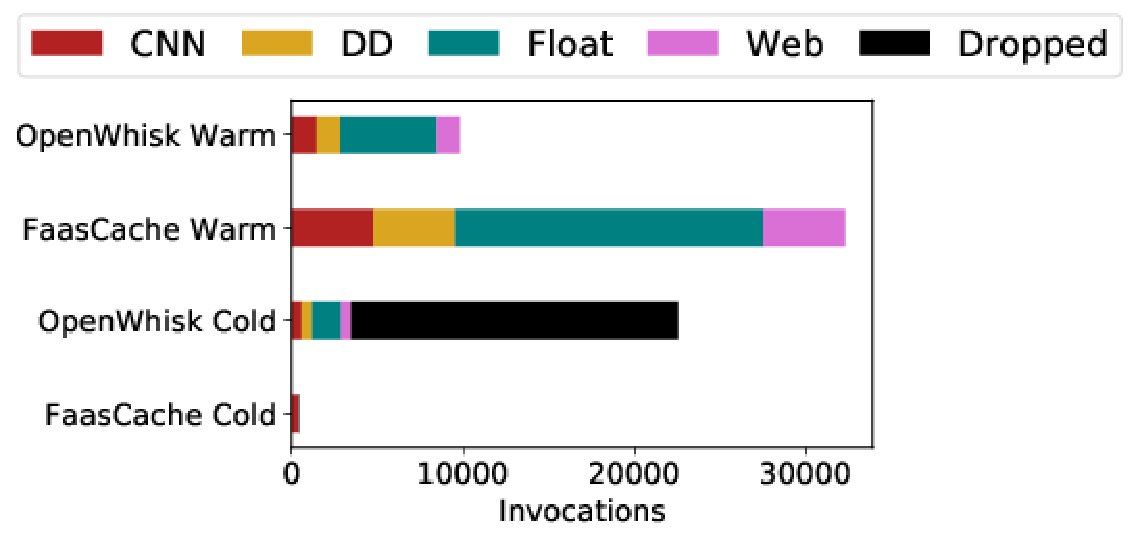
\includegraphics[width=0.3\textwidth]{../graphs/litmus_tests/faasbench_48_cold_hot-legend.pdf}}
\hfill 
  \subfloat[32 GB   \label{fig:faasbench-stacked-32}]
{  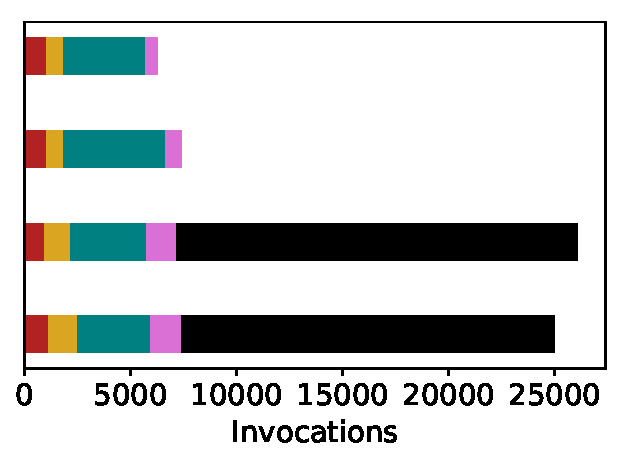
\includegraphics[width=0.17\textwidth]{../graphs/litmus_tests/faasbench_32_cold_hot.pdf}}
\caption{Impact of keep-alive on different function types.}
\label{fig:faasbench}
\end{figure}
\end{comment}

% Figure~\ref{fig:faasbench-stacked-32} shows the number of cold and dropped requests for the different functions, with a medium cache size of 32 GB.
% This setup is intended to evaluate our system in resource constrained environments.
% We see that dropped requests dominate, and FaasCache's more effective keep-alive serves 45\% of requests, while OpenWhisk only serving ~40\%.
% At the same time, warm starts improve 17\% using FaasCache.


Next, we use the skewed frequency workload and use functions from Table~\ref{tab:workloads} to evaluate the impact on real applications. 
%The impact on the different function performances can be seen in Figure~\ref{fig:faasbench}.
To generate the workload, the CNN, DD, and Web-serving functions have an inter-arrival time of 1500 ms, and the Floating-point function has a lower IAT of 400 ms. 
%
Figure~\ref{fig:faasbench} shows the breakdown of different function invocations for this workload on a 48 GB server.
Interestingly, OpenWhisk drops a significant number (50\%) of requests due to the its high cold start overheads.
FaasCache increases the warm requests by more than $2\times$. 
Interestingly, the \emph{distribution} of warm starts is also different. 
FaasCache's Greedy-Dual policy prioritizes functions with higher initialization times, but penalizes those with large memory footprints. 
Because the floating-point function has a high initialization overhead (Table~\ref{tab:workloads}), it sees a $3\times$ increase in hit-ratio compared to OpenWhisk.
\emph{In practical terms, the improvement in keep-alive results in a $6\times$ reduction in the application latency.
}
%The ML inference function has an 8\% lower warm hit rate than the other functions, as it gets de-prioritized because of it's high memory needs.


%When the cache size is increased to 48 GB (Figure~\ref{fig:faasbench-stacked-48}), FaasCache doesn't drop a single request, while OpenWhisk still can't serve 50\% of them.
%For the same workload, Figure~\ref{fig:faasbench-stacked-32} shows the distribution of cold and warm starts for a larger cache size of 32 GB.
%The number of warm starts increases by nearly 20\% compared to OpenWhisk.
% FaasCache's Greedy-Dual policy prioritizes functions with higher initialization times, the CNN function sees a 53\% higher warm starts, wheres Z function only sees X\% increase compared to OpenWhisk. 
% The floating point function has a very high initialization overhead (1.7 of the total 2 seconds), and thus sees its warm-start rate increase the most, by 40\%. 

\begin{comment}
At a smaller cache size of 32 GB shown in Figure~\ref{fig:faasbench-stacked-32}, the number of dropped requests dominate.
This setup is intended to evaluate our system in resource constrained environments.
FaasCache's more effective keep-alive serves 45\% of requests, while OpenWhisk drops nearly 60\%.
Warm-starts increase by 17\% with FaasCache. 
\end{comment}

\noindent \emph{\textbf{Result:} FaasCache can increase the number of warm-starts by $2\times$ to $3\times$ depending on the function initialization overheads and workload skew. This results in lower system load, which increases the number of requests FaasCache can serve by $2\times$.}

%\prat{CPU Graph not required, but just the average numbers will do.}

%%%%%%%%%%%%%%%%%%%%%%%%%%%%%%%%%%%%%%%%%%%%%%%%%%%%%%%%%%%%
\subsection{Effectiveness of Provisioning Policies}
\vspace*{\subsecspace}
All our previous results have been with a statically allocated server, and 
we now illustrate the effectiveness of our dynamic vertical scaling policy described in Section~\ref{subsec:dynamic}.
The goal is to dynamically adjust the cache size based on the workload. 
Our  policy seeks to keep the miss speed (cold starts per second) close to a pre-specified target. 
This is shown in Figure~\ref{fig:dynamic}---the target is 0.0015 misses per second. 
In this experiment, the cache resizing is done only when the miss speed error exceeds 30\%, and we can see that the cache size increases with the miss speed, and decreases with it. 
Without the dynamic scaling, a conservative provisioning policy would result in a constant, 10,000 MB size. 
In contrast, the average cache size with our proportional controller is less than 7,000 MB.
This 30\% reduction means that FaaS providers can reduce their provisioned resources without compromising on performance.
The freed-up resources can be used to accommodate additional cloud workloads (such as co-located VMs and containers). 
Our dynamic scaling is extremely conservative: increasing its agressiveness by reducing the error tolerance below 30\% will reduce  average server size,
%but cause a larger number of small memory-size  changes, which we wish to avoid.
but we seek to avoid the resultant small changes to memory-size to minimize fragmentation. 
%avoid why?? 

\begin{figure}[t]
    \vspace*{\myfigspace}
  \centering 
  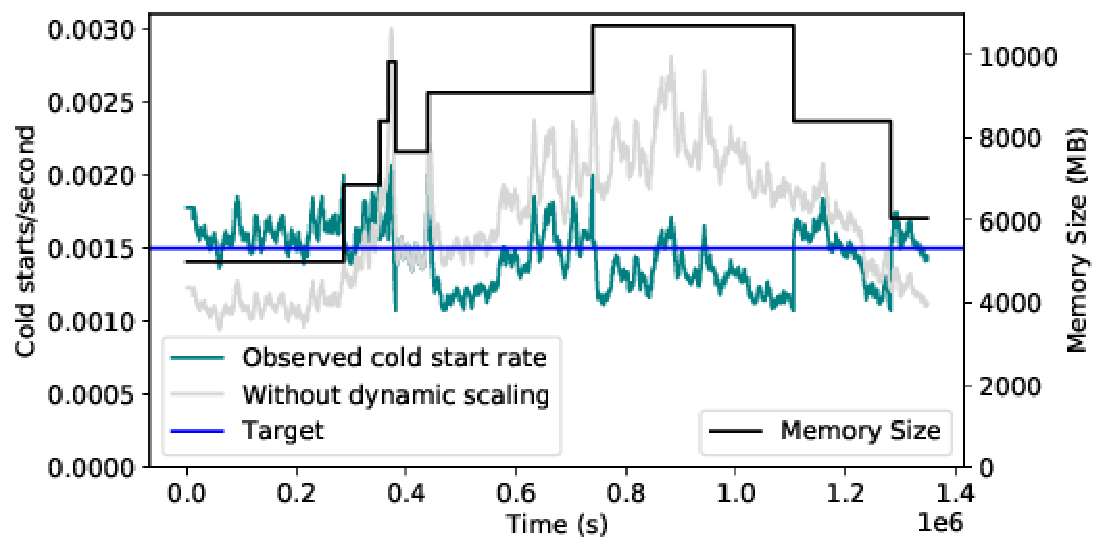
\includegraphics[width=0.47\textwidth]{../graphs/dyn-scale-392-b.pdf}
    \vspace*{\myfigspace}
  \caption{With dynamic cache size adjustment, the cold starts per second are kept close to the target (horizontal line), which reduces the average server size by 30\%. }
  \label{fig:dynamic}
  \vspace*{\myfigspace}
\end{figure}


%%% Local Variables:
%%% mode: latex
%%% TeX-master: "paper"
%%% End:
